%------------------------------------
% Dario Taraborelli
% Typesetting your academic CV in LaTeX
%
% URL: http://nitens.org/taraborelli/cvtex
% DISCLAIMER: This template is provided for free and without any guarantee 
% that it will correctly compile on your system if you have a non-standard  
% configuration.
% Some rights reserved: http://creativecommons.org/licenses/by-sa/3.0/
%------------------------------------

%!TEX TS-program = xelatex
%!TEX encoding = UTF-8 Unicode

\documentclass[10pt, a4paper]{article}
\usepackage{fontspec} 
\usepackage{tabularx}
% DOCUMENT LAYOUT
\usepackage{geometry} 
\geometry{a4paper, textwidth=5.5in, textheight=8.5in, marginparsep=7pt, marginparwidth=.6in}
\setlength\parindent{0in}

% FONTS
\usepackage[usenames,dvipsnames]{xcolor}
\usepackage{xunicode}
\usepackage{xltxtra}
\defaultfontfeatures{Mapping=tex-text}
%\setromanfont [Ligatures={Common}, Numbers={OldStyle}, Variant=01]{Linux Libertine O}
%\setmonofont[Scale=0.8]{Monaco}
%%% modified by Karol Kozioł for ShareLaTeX use
\setmainfont[
  Ligatures={Common}, Numbers={OldStyle}, Variant=01,
  BoldFont=LinLibertine_RB.otf,
  ItalicFont=LinLibertine_RI.otf,
  BoldItalicFont=LinLibertine_RBI.otf
]{LinLibertine_R.otf}
\setmonofont[Scale=0.8]{DejaVuSansMono.ttf}

% ---- CUSTOM COMMANDS
\chardef\&="E050
\newcommand{\html}[1]{\href{#1}{\scriptsize\textsc{[html]}}}
\newcommand{\pdf}[1]{\href{#1}{\scriptsize\textsc{[pdf]}}}
\newcommand{\doi}[1]{\href{#1}{\scriptsize\textsc{[doi]}}}
% ---- MARGIN YEARS
\usepackage{marginnote}
\newcommand{\amper{}}{\chardef\amper="E0BD }
\newcommand{\years}[1]{\marginnote{ #1}}
\renewcommand*{\raggedleftmarginnote}{}
\setlength{\marginparsep}{20pt}
\reversemarginpar

% HEADINGS
\usepackage{sectsty} 
\usepackage[normalem]{ulem} 
\sectionfont{\mdseries\upshape\Large}
\subsectionfont{\mdseries\scshape\normalsize} 
\subsubsectionfont{\mdseries\upshape\large} 

% PDF SETUP
% ---- FILL IN HERE THE DOC TITLE AND AUTHOR
\usepackage[%dvipdfm, 
bookmarks, colorlinks, breaklinks, 
% ---- FILL IN HERE THE TITLE AND AUTHOR
	pdftitle={BowenXu_cv},
	pdfauthor={BowenXu},
	pdfproducer={http://nitens.org/taraborelli/cvtex}
]{hyperref}  
\hypersetup{linkcolor=blue,citecolor=blue,filecolor=black,urlcolor=MidnightBlue} 

% DOCUMENT
\begin{document}
%{\LARGE Bowen Xu}\\[0.3cm]
%Ph.D Candidate\\
%School of Information System\\
%Singapore Management University\\
%, \texttt{310000}, China\\[.2cm]
%Phone: \texttt{+86 18268841236}\\
%Fax: \texttt{609-924-8399}\\[.2cm]
%Email: \href{mailto:maxxbw1992@gmail.com}{maxxbw1992@gmail.com}\\
%Supervisor: David Lo
%\textsc{url}: \href{http://www.ias.edu/spfeatures/einstein/}{http://www.ias.edu/spfeatures/einstein/}\\ 
%\vfill 
% Born:  October 04, 1992---Zhejiang Province, China\\
%Nationality:  Chinese


\begin{table}
\begin{tabularx}{\textwidth}{Xlr}

\begin{tabular}{@{}l@{}}
{\LARGE Bowen Xu}\\[0.3cm]
Ph.D Candidate\\
School of Information System\\
Singapore Management University\\
%, \texttt{310000}, China\\[.2cm]
%Phone: \texttt{+86 18268841236}\\
%Fax: \texttt{609-924-8399}\\[.2cm]
Email: \href{mailto:maxxbw1992@gmail.com}{maxxbw1992@gmail.com}\\
Supervisor: David Lo\\ \\ \\

{\LARGE Areas of specialization}\\[0.3cm]
Mining Software Repository\\
Program Analysis
\end{tabular}

&\raisebox{-0.5\height}{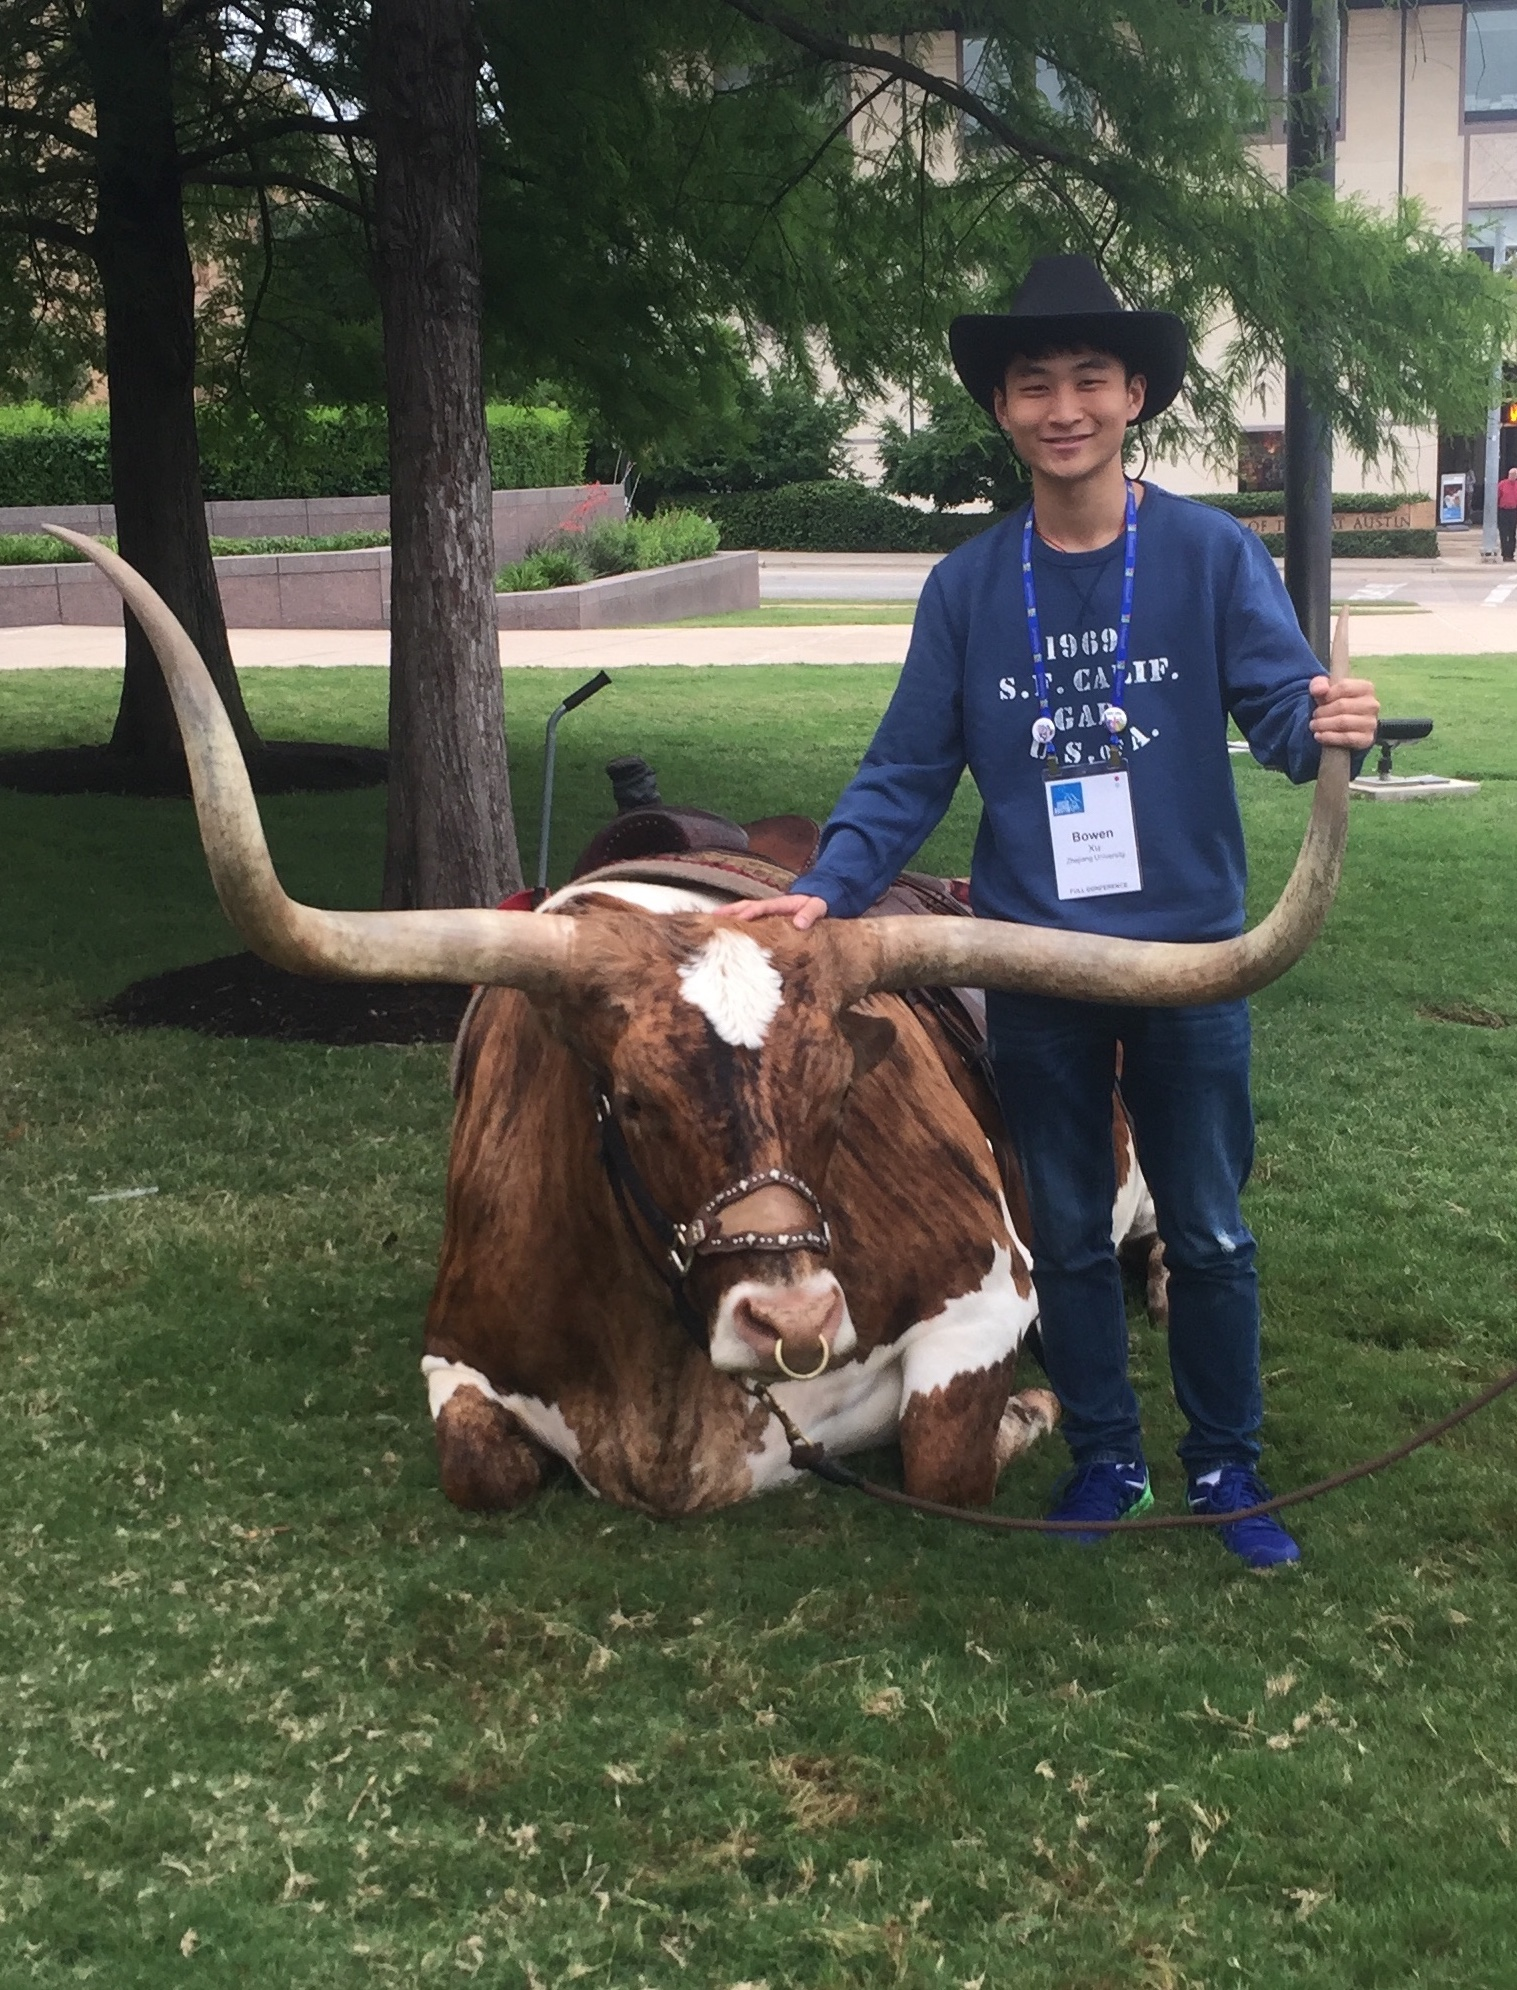
\includegraphics[scale=0.09]{me.jpg}}  

\end{tabularx}
\end{table}


%%\hrule
%\section*{Current position}
%\emph{Master Student}, Software Engineering Lab, Zhejiang University

%%\hrule
%\vspace{0.2cm}
%\section*{Areas of specialization}
%Mining Software Repository\\
%Program Analysis

%%\hrule
%\section*{Appointments held}
%\noindent
%\years{1903-1908}Swiss Patent Office, Bern\\
%\years{1908-1911}University of Bern\\
%\years{1911-1912}University of Zürich\\
%\years{1912-1914}Charles University of Prague\\
%\years{1914-1932}Prussian Academy of Sciences, Berlin\\
%\years{1920-1930}University of Leiden\\
%\years{1932-1955}Institute for Advanced Study, Princeton

%\hrule
\section*{Education}
\noindent
\years{\textbf{2017-Present}}\textsc{Ph.D Candidate} in School of Information System, Singapore Management University, Singapore\\
\years{\textbf{2014-2017}}\textsc{Master Degree} in School of Software Technology, Zhejiang University, China\\
\years{\textbf{2010-2014}}\textsc{Bachelor Degree} in College of Computer Science and Technology, Hunan City University, China


\section*{Publications}

\textbf{Conference Papers}

\noindent
\years{\textbf{ASE'17}}
\textbf{Bowen Xu}, Zhenchang Xing, Xin Xia, David Lo. ``AnswerBot - Automated Generation of Answer Summary to Developers' Technical Questions''.  \emph{32nd IEEE/ACM International Conference on Automated Software Engineering (ASE 2017)}. Accepted as a Full Paper.\\
\years{\textbf{ASE'16}}
\textbf{Bowen Xu}, Deheng Ye, Zhenchang Xing, Xin Xia, Guibin Chen, Shanping Li. ``Predicting Semantically Linkable Knowledge in Developer Online Forums via Convolutional Neural Network''.  \emph{31st IEEE/ACM International Conference on Automated Software Engineering (ASE 2016)}. Accepted as a Full Paper.\\
\years{\textbf{ASE'16}}
Guibin Chen, Chunyang Chen, Zhenchang Xing, \textbf{Bowen Xu}. ``Learning Dual-Language Vector Space for Domain-specific Cross-Lingual Question Retrieval''. \emph{31st IEEE/ACM International Conference on Automated Software Engineering (ASE 2016)}. Accepted as a Full Paper.\\
\years{\textbf{MSR'16}}
\textbf{Bowen Xu}, Zhenchang Xing, Xin Xia, David Lo, Qingye Wang, Shanping Li. ``Domain-Specific Cross-Language Relevant Question Retrieval''.  13th International Conference on Mining Software Repositories (MSR 2016). Accepted as a Full Paper. (Invited to Empirical Software Engineering Journal)\\
\years{\textbf{ICECCS'15}}
Yun Zhang, David Lo, Xin Xia, \textbf{Bowen Xu}, Jianling Sun, Shanping Li. ``Combining Software Metrics and Text Features for Vulnerable File Prediction''.  20th International Conference on Engineering of Complex Computer Systems (ICECCS 2015). Accepted as a Full Paper\\
\years{\textbf{APSEC'15}}
\textbf{Bowen Xu}, David Lo, Xin Xia, Ashish Sureka, Shanping Li. ``EFSPredictor: Predicting Configuration Bugs With Ensemble Feature Selection''. 22th Asia-Pacific Software Engineering Conference (APSEC 2015). Accepted as a Full Paper\\

\textbf{Journal Papers}

\years{\textbf{EMSE'17}}
\textbf{Bowen Xu}, Zhenchang Xing, Xin Xia, David Lo, Shanping Li. ``Domain-Specific Cross-Language Relevant Question Retrieval''. Empirical Software Engineering (EMSE). Accepted.\\

\vspace{0.5cm}
\textbf{Tool Demo Papers}

\years{\textbf{ESEC/FSE'17}}
\textbf{Bowen Xu}, Zhenchang Xing, Xin Xia, David Lo. ``XSearch: A DomainSpecific Cross-Language Relevant Question Retrieval Tool''. 11th joint meeting of the European Software Engineering Conference and the ACM SIGSOFT Symposium on the Foundations of Software Engineering. Accepted as a tool demo paper.\\


%\hrule

\section*{Grants, honors \& awards}
\noindent
\years{\textbf{2017}}Excellent Graduate of Zhejiang Province, Ministry of Education of the People's Republic of Zhejiang Province (top3\%), China,\\
%\years{2016}Scholarship for Outstanding Intern (top5\%), Insigma Hengtian Software Ltd, China\\
%\years{2015,2016}Outstanding Master Students (top10\%),  Zhejiang University, China\\
%\years{2015}Outstanding Graduate Student Cadres (top10\%), Zhejiang University, China\\
\years{\textbf{2014}}Scholarship of State Street (top5\%), State Street Corp, U.S.A\\
%\years{2014}Third Prize of the 2014 Ningbo Collegiate Programming Contest, Bureau of Education of Ningbo Municipality, China\\
%\years{2013}Scholarship for Outstanding Students, Second Prize (top10\%), Hunan City University,China\\
\years{\textbf{2012}}National Scholarship (top3\%), Ministry of Education of the People's Republic of China, China\\
%\years{2012}Scholarship for Outstanding Students, First Prize (top3\%), Hunan City University, China\\
%\years{2011}Scholarship for Outstanding Students, Third Prize (top30\%), Hunan City University, China


%\subsection*{Books}
%\noindent
%\years{1954}Einstein, Albert (1954), \emph{Ideas and Opinions}, New York: Random House, ISBN 0-517-00393-7

%\subsection*{Newspaper articles}
%\noindent
%\years{1940}Einstein, Albert, et al. (December 4, 1948), “To the editors", \emph{New York Times}\\
%\years{1949}Einstein, Albert (May 1949), “Why Socialism?", \emph{Monthly Review}.

%\section*{Teaching}

%...

%\hrule
%\section*{Service to the profession}

%...
%\vspace{1cm}
\vfill{}
%\hrulefill

%\begin{center}
%{\scriptsize  Last updated: \today\- •\- 
% ---- PLEASE LEAVE THIS BACKLINK FOR ATTRIBUTION AS PER CC-LICENSE
%Typeset in \href{http://nitens.org/taraborelli/cvtex}{
%\fontspec{Times New Roman}
%\XeTeX }\\
% ---- FILL IN THE FULL URL TO YOUR CV HERE
%\href{http://nitens.org/taraborelli/cvtex}{http://nitens.org/taraborelli/cvtex}}
%\end{center}

\end{document}